\documentclass{article}

% to give various notational syntax
\usepackage{amsmath,amsthm,amssymb, mathtools, enumerate, physics}

% for including images
\usepackage{graphicx}
\graphicspath{ {../../Images/} }
% Resize figures that are too wide for the page.
\makeatletter
\def\ScaleIfNeeded{%
  \ifdim\Gin@nat@width>\linewidth
    \linewidth
  \else
    \Gin@nat@width
  \fi
}
\makeatother
\let\oldincludegraphics\includegraphics
\renewcommand\includegraphics[2][]{%
  \oldincludegraphics[width=\ScaleIfNeeded]{#2}
}
%
%% for bibliography and citation
%\usepackage[square,compress]{natbib}
%\setcitestyle{super,comma}
%\bibliographystyle{unsrtnat}
%
%% for executing and including python code
%\usepackage{pythontex}
%
%% for defining lovely colors
%\usepackage{xcolor}
%\definecolor{light-gray}{gray}{0.95}
%
%% for syntax highlighting of non-python languages
%\usepackage{minted}
%\usemintedstyle[cpp]{manni}
%\newcommand{\cpp}[1]{\mintinline{cpp}{#1}}

% for linking sections of the document and table of contents
\usepackage{hyperref}
\hypersetup{
    colorlinks=true, %set true if you want colored links
    linktoc=all,     %set to all if you want both sections and subsections linked
    linkcolor=blue,  %choose some color if you want links to stand out
}


\newcommand{\nn}{\newline\newline}
\newcommand{\n}{\newline}
\newcommand{\bq}{\begin{equation}}
\newcommand{\eq}{\end{equation}}
\newcommand{\ba}{\begin{align}}
\newcommand{\ea}{\end{align}}
\newcommand{\bi}{\begin{itemize}}
\newcommand{\ei}{\end{itemize}}
\newcommand{\ct}[1]{\citep{#1}}

\newcommand*{\Perm}[2]{{}^{#1}\!P_{#2}}
\newcommand*{\Comb}[2]{{}^{#1}C_{#2}}




\begin{document}

\title{Bayesian Data Analysis}
\date{}
\maketitle

\textbf{Question:} Explain the Bayesian analysis approach in the framework of an ensemble of universes or a prior joint distribution. How do we choose among estimators in the Bayesian approach?
\n

\textbf{Question:} How is Bayes formula commonly applied in the context of real-world data analysis?
\n

\textbf{Conjugate Prior Problem}: Derive the full posterior distribution for $n$ data points that are modeled as i.i.d. with $X_i \sim \mathrm{Bernouilli}(\theta)$ where the prior on $\theta$ is U(0,1).
\n

\textbf{Clinical Analysis Problem}: We want to estimate the fraction, $\theta$, of the general population who will be improved by our drug - or in other words the probability that a random person will be improved. The data we have is that 18 people in a sample of 21 improved from receiving our drug (beyond their improvement from the placebo, which they were also given at a different time). Conduct a Bayesian analysis.
\n

\textbf{Problem:} In a 2D world a pole of height 1 has a laser affixed to it's top which is free to rotate in the plane (i.e. it can make any angle $\alpha$ it likes with the pole). The pole stands in the ground at at some location, and the x-axis runs perpendicular to the pole. The laser shoots light out of both ends and makes a spot on the ground at $X=x$ depending on its current angle (and of course where the pole is stuck in the ground). Given that the laser pole is fixed in the ground at an unknown location $\theta$ and we have a set of observations of laser spot location $\{X_i\}$. Proceed with a bayesian statisical analyis on $\theta$. 


\vspace{.3 in}

\tableofcontents

\section{Bayesian Analysis Framework}

This notecard is meant to be read after the notecard on the general Decision Theoretic Framework of Data Analysis. At various points throughout I will include \emph{[asides]} which connect what I am saying back to that  framework, but this notecard focuses on a different mental representation which I also find helpful: the sample space of universes. 
\nn

Our goal is to estimate the true value of some parameter, $\theta$, which parameterizes a distribution that is generating data that we are observing.  \emph{[So this is a density or function estimation DP.]} The essence of a Bayesian analysis for this task is: what is the probability for $\theta$ to have various values, \textit{given} that we have observed some particular value of the data, and having some prior belief about $\theta$ before the experiment. \emph{[Our DP will involve obtaining a probability distribution on the truth space.]}
\nn

Our prior beliefs about $\theta$ can be written as a probability distribution over the possible values, which is called the \textbf{prior}. It can be helpful to visualize a sample space that is a huge ensemble of universes, each universe having one true value of $\theta$ and one value of the experimental outcome $X$ (the data). In this SS the number of universes with a specific value $\theta_0$ is proportional to our prior beliefs about how likely it is that $\theta_0$ is the true value of our universe. Then within each subset of specific $\theta_0$ values, the proportion of that set having $X=X_0$ reflects how likely the $\theta_0$ distribution is to generate the data $X_0$.  A priori we believe our universe is one of the universes in this SS, and without any data each one is equally likely as far as we can tell. An obvious way to partition this sample space is by value of $\theta$, and we are interested in which partition our universe lies in. \emph{[The sample space visualization helps to understand why this DP is a sensible thing to do in terms of conditional probability.]}
\nn
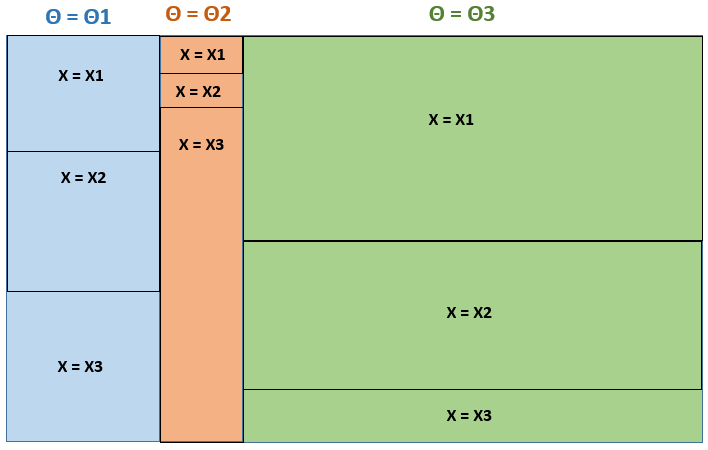
\includegraphics{universeSS}
\nn

Now the question arises, \textit{given} that we observed a specific experimental outcome, $X$, what is the probability that our universe is in each partition $\Theta_i$? (Of course $\theta$ could be continuous, but it is more helpful to picture the discrete case).
\begin{align}
P(\Theta_i|X) = \frac{P(\Theta_i\cap X)}{P(X)}, \textrm{ from the definition of conditional probability,}\\
= \frac{P(\Theta_i)P(X|\Theta_i)}{\sum_jP(\Theta_j)P(X|\Theta_j)}, \textrm{ from Bayes formula}.
\end{align}

We know the various $P(\Theta_i)$ because these are from our prior beliefs. The $P(X|\Theta_i)$ we should calculate based on the mechanism for how this data arises. Recall the goal of this analysis was to estimate the value of $\theta$ which is parameterizing this generating mechanism - the set of specific functions from all the possible$\theta$ values is called the model. The specific form of the generating mechanism enables us to calculate a probability distribution over $X$ for a given value of $\theta$. For instance if your model is that your $n$ data points are i.i.d. all Bernoulli($\theta$) and you can readily calculate the probability of data $X$ being $s$ successes and $n-s$ failures given some $\theta$.
\nn

In the language of Bayesian analysis, from the expression above we say:
\begin{align}
P(\Theta_i|X) = \frac{P(\Theta_i)P(X|\Theta_i)}{\sum_jP(\Theta_j)P(X|\Theta_j)},\\
P(\Theta_i|X) \propto P(\Theta_i)P(X|\Theta_i)\\
\textrm{Posterior}\propto \textrm{Prior}*\textrm{Likelihood}.
\end{align}
So the prior is a probability density over $\theta$ and the \textbf{likelihood} is a function of $\theta$ that gives a probability density over $X$. The \textbf{posterior} is the distribution which describes our new beliefs about how likely different $\theta$s are now that we have observed this particular data.
\nn

You could also say that your prior beliefs about the world are represented by a joint distribution over $\theta$ and $X$ whose weights come from the your statement about the form of the data-generating mechanism (model) and your belief about how likely different $\theta$ values are: $P(\theta, X) = P(\theta)P(X|\theta)$. The Bayesian analysis then would consist of calculating a particular conditional distribution $P(\theta|X=X_{\text{observed}})$ from this joint distribution. For example: Suppose we have a prior belief about the joint distribution of heights of twins, then we measure the height of Twin1 and we are interested in updating our beliefs about the height of the Twin2. In this case our prior belief about height of Twin2 is just the marginal density of the joint distribution, a function of $h_2$. The model for our data $h_1$ is the conditional probability $P(h_1|h_2)$ from the joint distibution.
\nn

\subsection{Estimators in Bayesian Analysis}
Now if your Bayesian analysis was aimed at estimating the parameters of a population density, your posterior allows you to make statements about how likely different values for future samples are. Similarly if your analysis was estimating the parameters or form of a functional relationship between some observables, $\{X_i\}$ and some response $Y$ then for future measurements of new $\{X_i\}$ your posterior gives you statements about how likely different values of $Y$ are. But often it is desirable to have a method for choosing one representative density or function to move forward with. What should be the method for choosing? \emph{[A final step in the DP.]} For Bayesians it is common to want the method which minimizes the expectation of the loss function over the ensemble of universes sample space i.e. over the joint distribution on $(\theta, X$). This is equivalent to wanting the method which minimizes the \textbf{Bayes Risk}, this method is called the \textbf{Bayes Estimator} of the system. If your loss function is squared error between the true and the representative parameter values, the Bayes Estimator is to choose the representative whose parameter has the value which is the mean value of the posterior on $\theta$. If instead your loss is relative entropy between the true distribution and the representative distribution then the Bayes Estimator is to use a representative which is the posterior-weighted mixture of the possible densities / functions. If you have 0/1 loss (0 if you choose the true value correctly, 1 otherwise) then the Bayes Estimator is choosing the posterior mode (the most probable point), and to the extent that you have a highly peaked loss function this may be a good DP. This procedure is called Maximum A Posteriori (MAP). For more on Loss, Risk and Estimators, see the DTFoA notecard.

\section{Bayesian Analysis in Practice}
It is possible to do some Bayesian analyses by hand with pencil and paper analytical calculation. In the real world however most Bayesian analyses rely on numerical techniques like MCMC to algorithmically sample from the posterior, which allows us to answer questions about the (approximate) probability of various outcomes without explicitly having to calculate the normalization factor of the posterior. But in the case of analytical calculation it is often very convenient if you can use a conjugate prior. 

\subsection{Conjugate Priors}
\textbf{For a given functional form of model (and thus likelihood), the conjugate prior is a family of distributions such that when the prior is chosen to be a member of the family, the posterior also will be a (different) member of that family.} The value of the distribution parameter for the posterior is typically a simple function of the value for the prior distribution and the data. Often this function comprises a weighted average of some characteristic from the prior and some statistic from the data, where the weighting is skewed toward the prior if the prior is highly peaked, but skewed toward the data if $n$ is large or the data are low-variance.
\n

Two useful examples are:
\begin{enumerate}
\item If $\{X_i\}$ i.i.d. Bernoulli($\theta$), then the conjugate prior is the $\mathrm{Beta}(\alpha, \beta)$ distribution.
\item If $\{X_i\}$ i.i.d. N($\mu, \sigma_0$), where $\sigma_0$ is known, then the conjugate prior is also a normal distribution.
\item If $\{X_i\}$ i.i.d. N($\mu_0, \sigma$), where $\mu_0$ is known, then the conjugate prior is a gamma distribution.
\end{enumerate}

A possibly useful trick is that actually a uniform distribution is equivalent to a Beta(1,1) so that for sequences of i.i.d. Bernoulli RVs with uniform prior, the posterior will be Beta. 

\subsection{Conjugate Prior Problem}
If we have $n$ data points of which $p$ are successes and the rest are failures, a reasonable model would be that the points are i.i.d. with $X_i \sim \mathrm{Bernouilli}(\theta)$. The likelihood would then the be the probability of getting $p$ successes AND $n-p$ failures: $L(\theta) = \theta^p (1-\theta)^{n-p}$. If we take the prior as $\theta$ is U(0,1) then a straightforward Bayesian analysis says the posterior is proportional to the likelihood times the prior:
\begin{align*}
f(\vec{X} | \theta) \propto \theta^p (1-\theta)^{n-p} * 1.
\end{align*}

We would normally now need to calculate the normalization of the posterior by integrating, or just do some Monte Carlo sampling of the non-normalized expression. However we can instead note that for a model of $n$ i.i.d. Bernoulli draws, the conjugate prior is a Beta distribution, and in fact the uniform distribution is a special case of a Beta: U(0,1) = Beta(1,1). Now we know immediately that the posterior is $f(\vec{X}|\theta)$ is the distribution Beta($1+p, 1+(n-p)$).


\section{Clinical Analysis Problem}
We want to estimate the fraction, $\theta$, of the general population who will be improved by our drug - or in other words the probability that a random person will be improved. It should also be thought of as figuring out which distribution (parameterized by $\theta$) we believe generates this data in the real world. The data we have is that 18 people in a sample of 21 improved from receiving our drug (beyond their improvement from the placebo, which they were also given at a different time). We want to calculate a new probability for $\theta$ to have various values, \textit{given} that we have observed this particular data, and having some prior belief about $\theta$ before the experiment. 
\nn
A reasonable model for this data is that each person is independent of others and has a success probability $\theta$ for the treatment. Thus we would expect $X\sim B(21,\theta)$. 
\nn
There might be many reasonable priors. If we choose a uniform prior $\theta \sim U(0,1)$ then the posterior will have a shape identical to the likelihood (binomial). 


\section{Problem: Laser Pole Density}

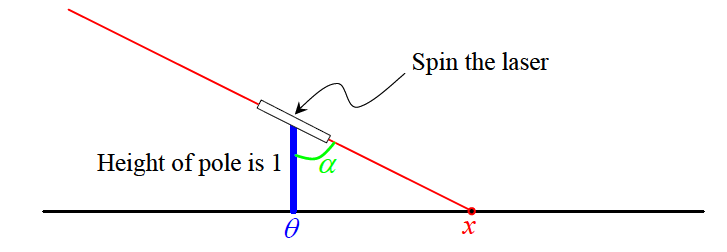
\includegraphics{laserpole} 
The general framework for the bayesian analysis is that we must have a prior on the $\Theta$s and we must figure out what the likelihood function is. Then we can compute the non-normalized posterior on $\Theta$. In this case the likelihood function is the probability density to observe $X=x$ given that $\Theta=\theta$ - so we must first ascertain something about the probabilities on $X$.
\n

We will first conduct an analysis assuming $\Theta =0$ i.e the pole is stuck in the ground at the origin. We know the pdf $A \sim U(-\pi/2,\pi/2)$ and that $X=tan(A)$, but now we are interested in the pdf of $X$ - what will be the relationship between these two? Refer to the above problem for a general discussion of getting the pdf for an RV which is a function of another RV whose pdf you already know. Using the method of working through the CDFs we have:

\begin{equation}
F(x) = P(X \leq x) = P(tan(A) \leq x) = P(A \leq tan^{-1}(x)).
\end{equation}
Since $A$ is uniform over an interval of length $\pi$ it is straightforward to calculate that
\begin{align*}
F(x) = P(A \leq tan^{-1}(x)) = \bigg(tan^{-1}(x) - (-\pi/2)\bigg)\frac{1}{\pi}\\
\implies f_X(x) =\pi( \frac{d}{dx}tan^{-1}(x))=\frac{1}{\pi(1+x^2)}.
\end{align*}
This is actually a well-known distribution called the Cauchy distribution - it is highly peaked in the center but with fatter tails than the normal distribution. We have some physical intuition for this peak as any angle less than 45 degrees with the pole gets mapped to a finite= segment on the x-axis while the the angles greater than 45 degrees get mapped to an infinite length of x-axis. Since these two categories for solid angle carry the same probability weight, we should expect the probabilty weight of $X$ to get diluted down as $x$ increases. 
\n

Now we return to the case of not knowing where the pole is stuck in the ground. Physically we can picture clearly that shifting the laser pole a certain distance from the origin is just going to shift the mapping of the density on X, namely
\begin{equation}
f_{X|\Theta}(x|\theta) \rightarrow f_X(x-\theta) = \frac{1}{\pi(1+(x-\theta)^2)}.
\end{equation}
To understand the minus sign imagine what the density at $x=0$ should do as we shift the pole rightward. I've written it as a conditional density in the spirit of imagining $\Theta$ and $X$ as existing in a joint distribution. We can now calculate the likelihood $L(\theta ; \{X_i=x_i\})=\sum_i f_{X|\Theta}(x_i|\theta)$. 

\end{document}